\documentclass[12pt]{article}
\usepackage[letterpaper, top=1.25in, bottom=1.25in, left=1in, right=1in]{geometry}
\usepackage{fancyhdr} % http://ctan.org/pkg/fancyhdr
\usepackage{hyperref}
% \usepackage{xcolor}
\usepackage{graphicx}
\usepackage{indentfirst}
\usepackage[export]{adjustbox}

% % % % % % % % % % % % 
% Citation formatting %
% % % % % % % % % % % % 

\usepackage[style=ieee]{biblatex}
\addbibresource{sources.bib}

% % % % % % % % %
% Hyperlinking  %
% % % % % % % % %

\hypersetup{
    colorlinks=false, % set true if you want colored links
    linktoc=all,     % set to all if you want both sections and subsections linked
    % linkcolor=black,  %c hoose some color if you want links to stand out
    % citecolor=black
    % urlcolor=black
}

% % % % % % % % % % % % % % % %
% Global title, author, date  %
% % % % % % % % % % % % % % % %

\title{Exploring Smart Sensor Systems}
\author{Nathan Quadras \& Kosta Sergakis}
% \author1{Quadras \& Sergakis}
% \date{\today}
\date{April 28, 2025}
\makeatletter
\let\runauthor\@author
\let\runtitle\@title
\let\rundate\@date
\makeatother

% % % % % % % % % % %
% Header and Footer %
% % % % % % % % % % %

\pagestyle{fancy} % change page style to fancy
\fancyhf{} % clear header/footer
\setlength{\headheight}{15pt}
\fancyhead[L]{Quadras \& Sergakis}
\fancyhead[C]{\runtitle}
\fancyhead[R]{\rundate}
\fancyfoot[C]{\thepage} % \fancyfoot[R]{\thepage}
\renewcommand{\headrulewidth}{0.4pt} % default \headrulewidth is 0.4pt
\renewcommand{\footrulewidth}{0.4pt} % default \footrulewidth is 0pt

% \usepackage{natbib}
\begin{document}

    % % % % % % % %
    % Title Page  %
    % % % % % % % %
    
    \begin{titlepage}
        \begin{center}
            \vspace*{1.5cm}
            
            \textbf{\runtitle}
            
            \vspace{1cm}
            
            An exploration of:\\
            \vspace{0.25cm}
            Slip Angle Sensors
                
            \vspace{1cm}
            
            \textbf{\runauthor}
            
            \vfill  
            
            \vspace{1cm}

            
\includegraphics[width=0.3\textwidth]{resources/michigan-state-logo-png-transparent.png}
                
            Electrical and Computer Engineering\\
            Michigan State University\\
            East Lansing, Michigan\\
            \rundate
                
        \end{center}
    
    \end{titlepage}


    % % % % % % % % % % %
    % Table of Contents %
    % % % % % % % % % % %

    \setcounter{secnumdepth}{0} % removes section numbers
    % \maketitle
    
    \tableofcontents
    
    \newpage

    \section{Introduction}
        
    Vehicles are more attainable than ever and are advancing quickly. Modern cars 
    are equipped with sophisticated systems that enhance performance, safety, and driver 
    comfort. Vehicle dynamics is a tremendous topic and an area of growing interest, especially 
    as more automated driving technologies emerge. Vehicle dynamics is the study of vehicle 
    motion in relevant user operations \autocite{Jacobson_2016}, which encompasses factors like kinematics, forces, 
    and moments acting on a vehicle during acceleration, braking and steering. The core of vehicle 
    dynamics involves the following primary aspects: the mechanisms that disturb a vehicle’s state 
    (inputs) and the mechanisms through which the vehicle responds (outputs). Arguably the most 
    critical aspect of vehicle dynamics is tire behavior, specifically how a tire generates lateral 
    force during cornering. Central to this behavior is the concept of slip angle – the difference 
    between the direction a vehicle is traveling and the direction that the body of the vehicle is 
    pointing (heading vs. true heading) \autocite{Racelogic_2015}. Understanding slip angle is essential for analyzing 
    handling characteristics, improving stability control systems, and optimizing driver feedback.
        
        \subsection{Vehicle Dynamics}

        Performance driving, autonomous driving and commuter driving all require the same characteristic: 
        control. Controllable vehicles are what makes rapid maneuvers possible. On the other hand, the required 
        motion must be stable to maintain directional stability under disturbances \autocite{MMM}. 

        \begin{center}
            \vspace{0.5cm}

            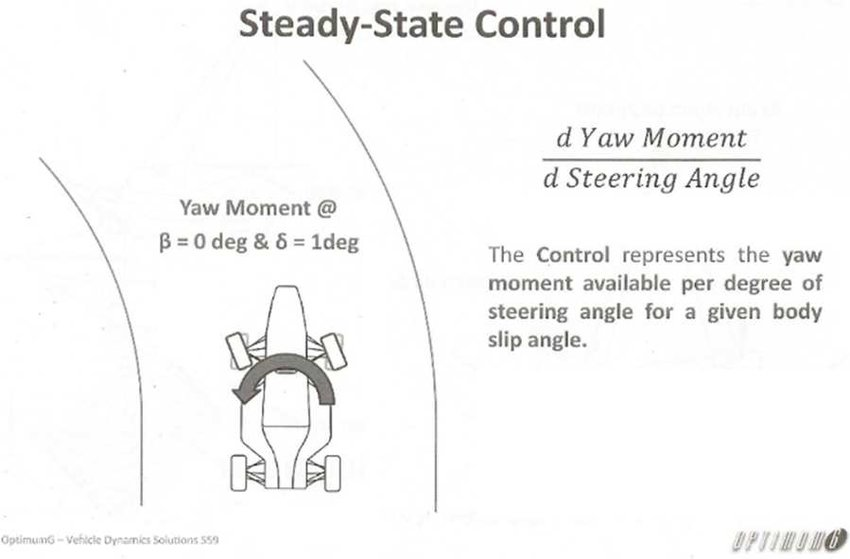
\includegraphics[width=0.7\textwidth]{resources/Defining-of-control-Claude-Rouelle-Applied-VD-seminar.png}

            \vspace{0.5cm}

            \textbf{Figure 1: Definition of Control} \autocite{MMM}
            \label{control}
        
        \end{center}

        \begin{center}
            \vspace{0.5cm}

            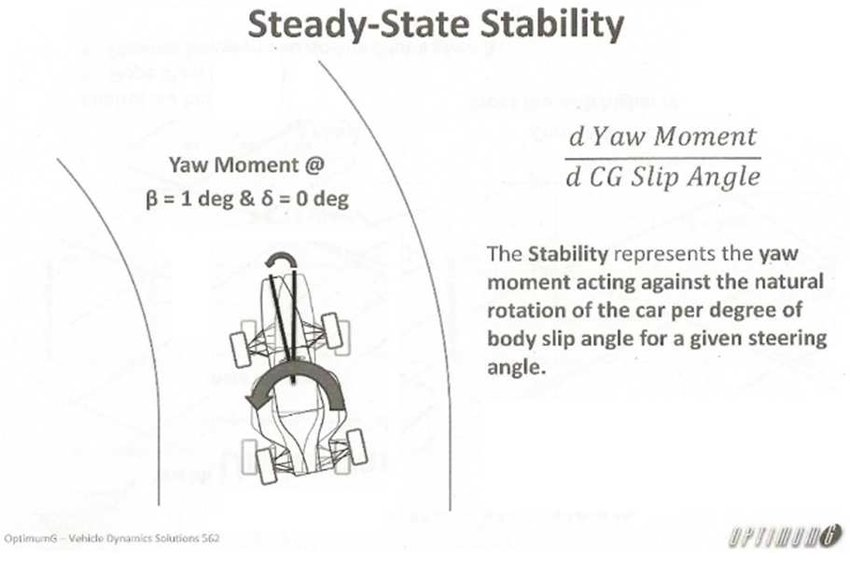
\includegraphics[width=0.7\textwidth]{resources/Defining-of-stability-Claude-Rouelle-Applied-VD-seminar.png}

            \vspace{0.5cm}

            \textbf{Figure 2: Definition of Stability} \autocite{MMM}
            \label{stability}
        
        \end{center}

        It is crucial to define the tractive limit of the vehicle, or the “safety margin” to determine the range of 
        possible motions that the vehicle can produce while maintaining stability \autocite{MMM}. Slip angle is incredibly important 
        because it enables the concepts mentioned above. In other words, slip angle determines vehicle maneuverability. If 
        slip angle is observed, various states of the vehicle can be determined. 

        % \begin{center}
        %     \vspace{0.5cm}

        %     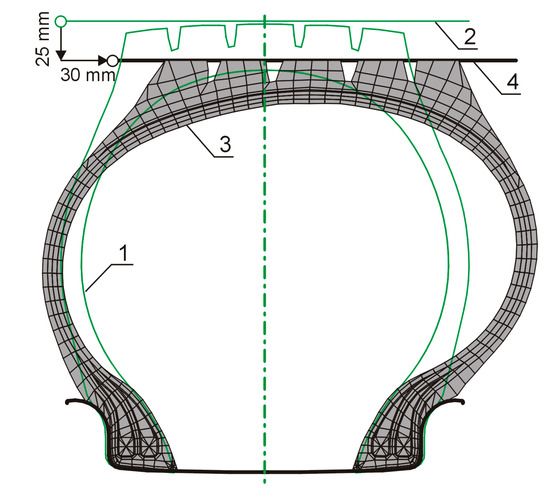
\includegraphics[width=0.5\textwidth]{resources/applsci-10-04326-g009-550.jpg}

        %     \vspace{0.5cm}

        %     \textbf{Figure 3: Tire Deformation} \autocite{app10124326}
        %     \label{tire_deformation_1}
        
        % \end{center}

        \begin{center}
            \vspace{0.5cm}

            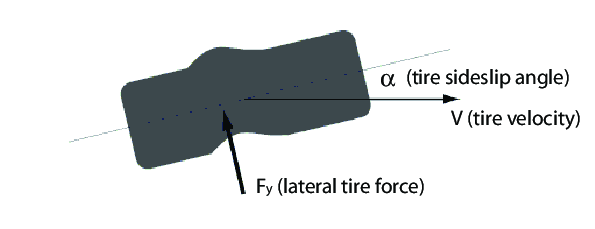
\includegraphics[width=0.8\textwidth]{resources/Lateral-tire-deformation.png}

            \vspace{0.5cm}

            \textbf{Figure 3: Tire Deformation} \autocite{inproceedings}
            \label{tire_deformation_2}
        
        \end{center}

        \begin{center}
            \vspace{0.5cm}

            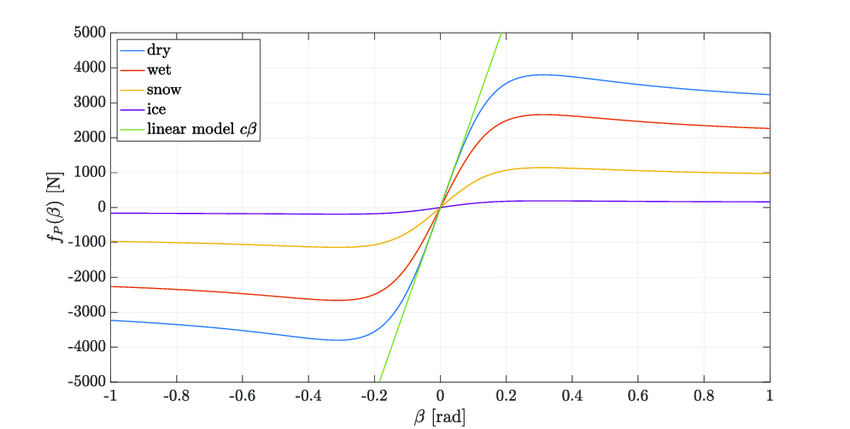
\includegraphics[width=1\textwidth]{resources/Pacejkas-tire-model.png}

            \vspace{0.5cm}

            \textbf{Figure 4: Example Pacejka Tire Model} \autocite{pacejka}
            \label{pjka}
        
        \end{center}

        \begin{center}
            \vspace{0.5cm}

            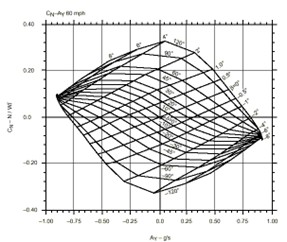
\includegraphics[width=0.5\textwidth]{resources/tn_MMM807.jpg}

            \vspace{0.5cm}

            \textbf{Figure 5: MMM} \autocite{Milliken_Research_Associates}
            \label{MMMa}
        
        \end{center}

        A common way to observe/determine the limits of a vehicle is through a Yaw Moment Diagram, or the MRA Moment Method 
        (MMM) \hyperref[MMMa]{[Figure 5]} \autocite{Milliken_Research_Associates}. A critical component of the Yaw Moment Diagram would be the quantification of the forces necessary to hold 
        a vehicle through a turn. As shown in  \hyperref[tire_deformation_2]{Figure 3}, a primitive to determining the lateral force of a tire is the slip angle. 
        Pacejka’s formula can display the relationship between slip angle and lateral tire force as shown in \hyperref[pjka]{Figure 4}. Ultimately, 
        the goal is to determine the limits of the vehicle to prevent drivers from reaching the point of no return; a loss of 
        stability, leading to control being removed from the driver.

        \subsection{Overview \& Motivation}
        
        This smart system focuses on real-time slip angle estimation and control for ground vehicles. Accurate knowledge of 
        slip angle enables Advanced Drive-Assistance Systems (ADAS), traction control, and autonomous driving algorithms to make 
        more informed decisions when navigating corners, avoiding obstacles, or maintaining control on low-friction surfaces. 
        
        The motivation for this system stems from the growing demand for safer and more responsive vehicles in both human-driven 
        and autonomous applications. While modern vehicles are equipped with various sensors, slip angle is notoriously expensive 
        to measure directly due to the niche, specialized equipment involved. By designing a smart system capable of observing slip 
        angle in real-time using accessible components, this solution offers a cost-effective and scalable method to improve vehicle 
        safety, performance, and driver confidence across a wide range of driving conditions. 

    \section{System Level Design}
        
        \begin{center}
            \vspace{0.5cm}

            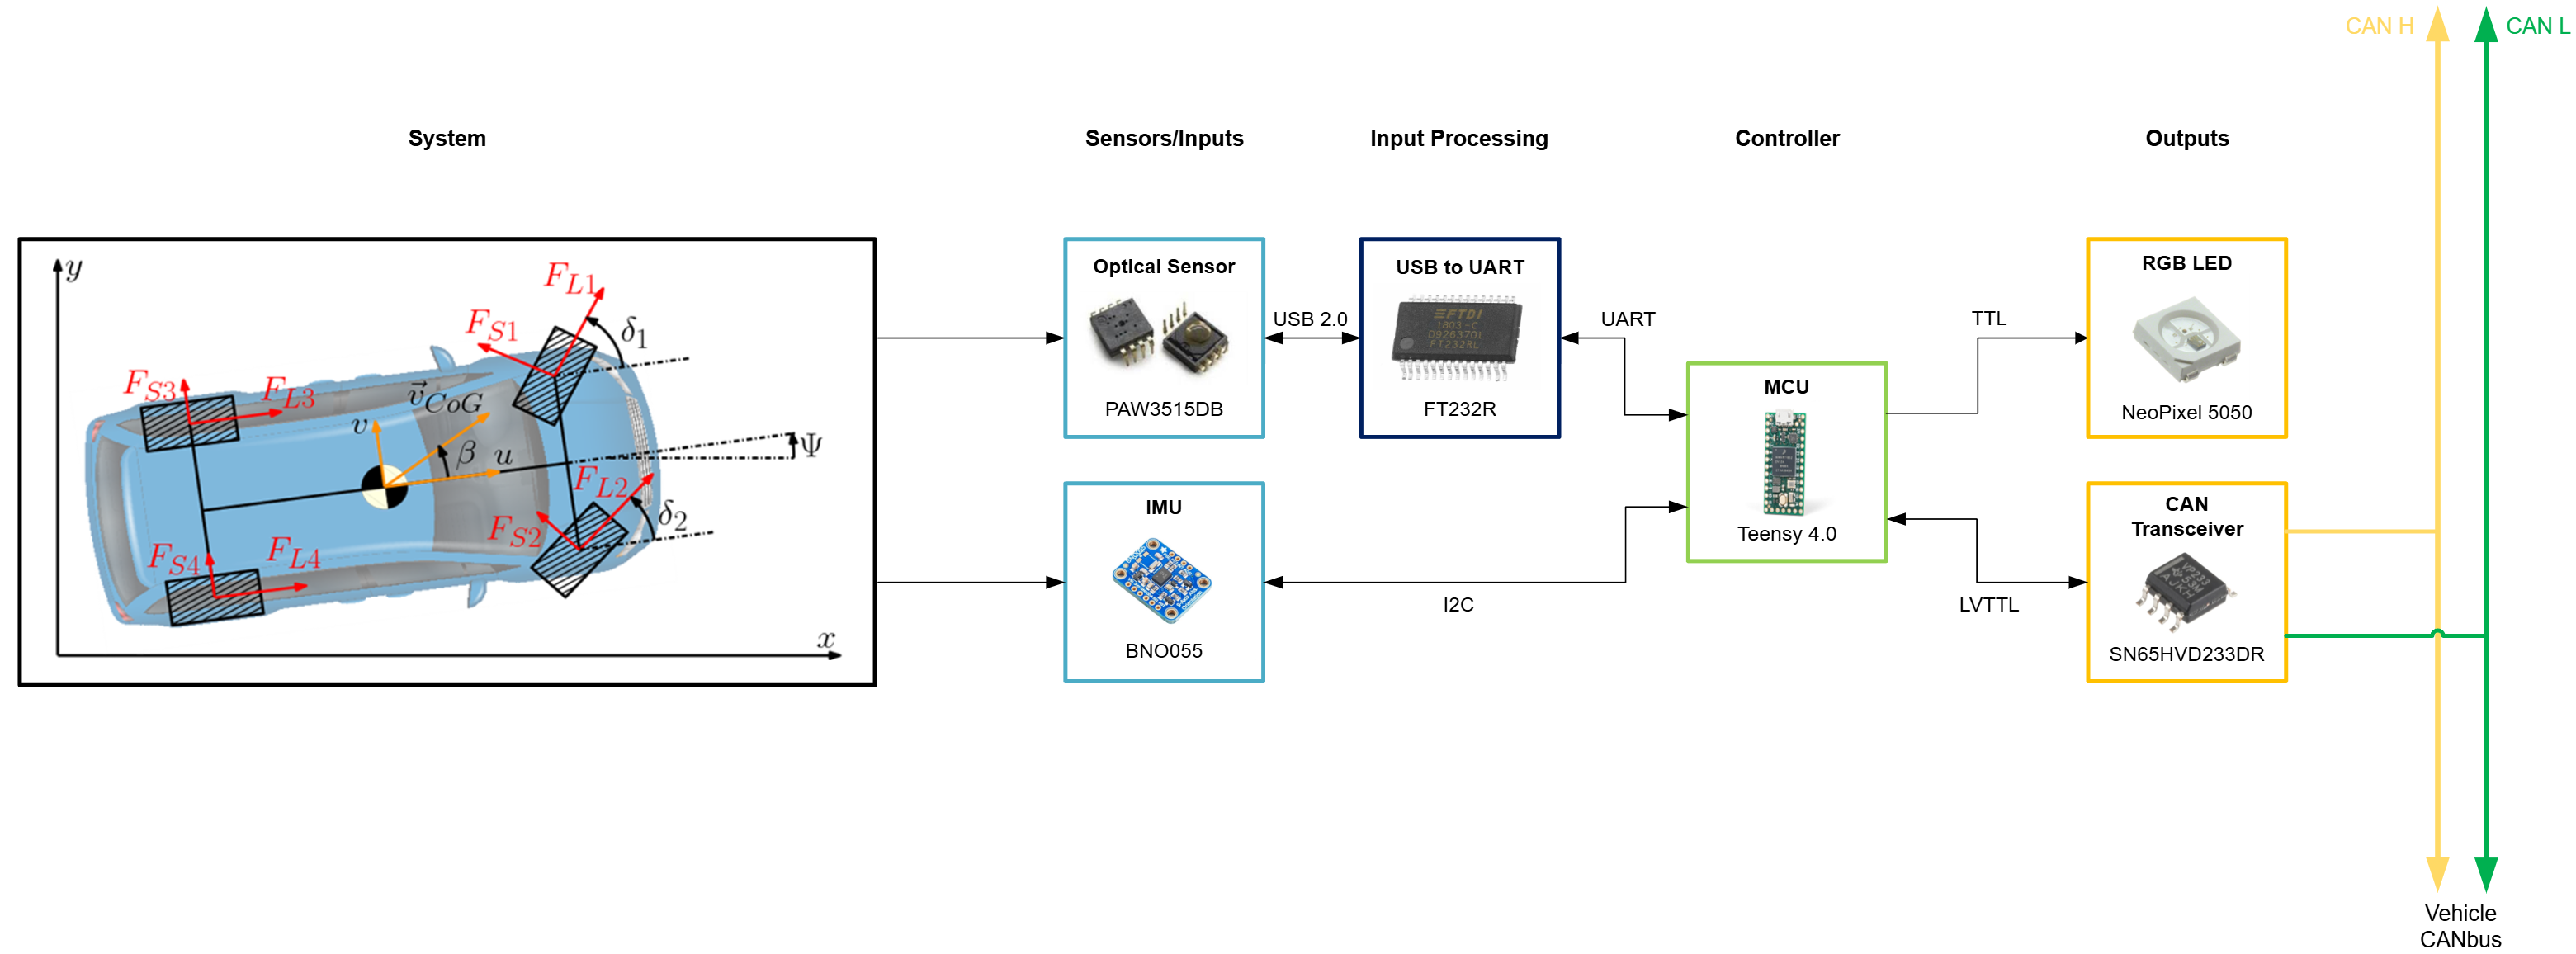
\includegraphics[width=1\textwidth]{resources/Screenshot 2025-04-27 181552.png}

            \vspace{0.5cm}

            \textbf{Figure 6: Hardware Diagram}
            \label{hd}
        
        \end{center}

        % words and text

        % \begin{center}
        %     \vspace{0.5cm}

        %     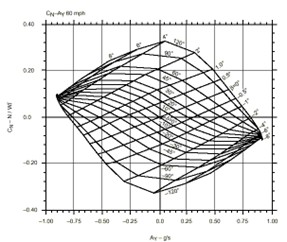
\includegraphics[width=0.5\textwidth]{resources/tn_MMM807.jpg}

        %     \vspace{0.5cm}

        %     \textbf{Figure 7: Intended Application}
        %     \label{ia}
        
        % \end{center}
        
        \subsection{Microcontroller (Teensy 4.0)}

            The Microcontroller Development Board selected for this project is the Teensy 4.0, which is powered by NXP’s i.MX RT1062 
            microcontroller. This device boasts an Arm Cortex‑M7 core running at 600 MHz, one of the fastest Cortex‑M MCUs available. 
            The core is accompanied by a hardware floating‑point unit (FPU) and digital signal processing (DSP) extensions, making it 
            ideally suited for real‑time control, signal processing, and multimedia applications. 

            The Teensy is equipped with 1984K Flash, 1024K RAM (512K tightly coupled), 1K EEPROM (emulated) and supports a rich set of 
            peripherals. It has 40 of these digital I/O pins with 14 analog input pins with up to 12-bit resolution, and 31 digital pins 
            with PWM capabilities. It supports standard communication interfaces like I2C, UART, and SPI, along with more advanced options 
            such as USB 2.0 OTG, CAN, and Ethernet. It also includes general-purpose timers, using the inbuilt Systick on the core, RTC, and 
            a watchdog timer which enables easy use of interrupts, time-based operations, date-time access, and system monitoring, offering 
            flexibility for a wide range of embedded system designs.

            Programming the teensy can be done through a variety of mediums including the Arduino IDE (via the Teensyduino plug‑in) or in 
            PlatformIO, providing a rapid, user‑friendly workflow. For in‑depth development and troubleshooting, the i.MX RT1062 implements 
            ARM CoreSight with SWD/JTAG access. Additionally, its Nested Vectored Interrupt Controller (NVIC) supports deterministic and 
            priority-based interrupt handling, allowing for example, slip angle computations at 1 kHz to interrupt lower priority routines with 
            negligible overhead, while optional JTAG pads enable real‑time trace capture and hardware breakpoints for advanced optimization. 

            Together, these capabilities make the Teensy 4.0 and, by extension, the i.MX RT1062 an exceptionally powerful yet compact platform 
            for our slip‑angle detection system and for embedded systems development in general. 

        \subsection{Optical Sensor (PAW3515DB)}
            
            \subsubsection{USB to UART (FT232R)}
                FTDI is pretty sick

        \subsection{Inertial Measurement Unit (BNO055)}

            The BNO055 is a compact, all-in-one 9-axis inertial measurement unit (IMU) developed by Bosch that combines combining a 3-axis 16-bit 
            gyroscope, a 3-axis 14-bit accelerometer, and a 3-axis full performance magnetometer, along with a built-in ARM Cortex-M0+ processor 
            for onboard sensor fusion. The sensor supports various power management modes (normal, low power, suspend), programmable acceleration 
            and gyroscope ranges (±2g to ±16g and ±125°/s to ±2000°/s respectively), and is capable of motion-triggered interrupt generation. 
            Unlike raw IMUs that require external processing, the BNO055 outputs fully fused orientation data including quaternions, Euler angles 
            (roll, pitch, yaw), linear acceleration, gravity vectors, and heading. With its ability to provide accurate and drift-compensated yaw 
            angle measurements, and easy interfacing through I2C or UART, the BNO055 is well-suited for determining the heading direction of a vehicle. 

        \subsection{RGB LED (NeoPixel 5050)}

            Here an RGB can be utilized as a status indicator for the device. When the system is powered on and functioning normally, the LED displays 
            green, signaling active and healthy operation. If an error is detected, such as communication failure or sensor malfunction, the LED switches 
            to red to alert the user. When the device is in an idle or powered-off state, the LED remains off, conserving power and clearly indicating inactivity. 

            ALSO TALK ABOUT RUNTIME STUFF

    \section{Software Design}

        \begin{center}
            \vspace{0.5cm}

            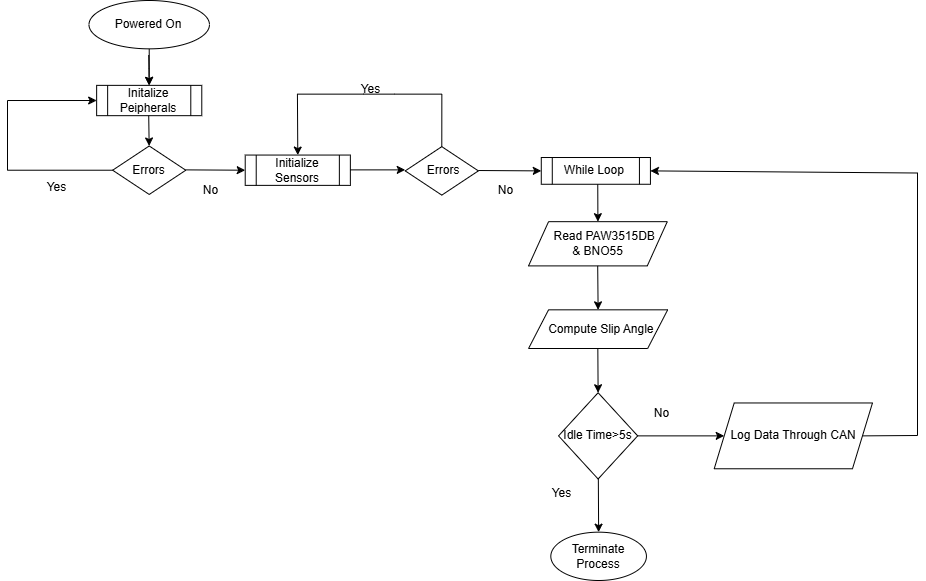
\includegraphics[width=1\textwidth]{resources/softwarediagram.png}

            \vspace{0.5cm}

            \textbf{Figure 7: High-Level Software Design}
            \label{sd}
        
        \end{center}

        On powering up the system, the firmware first configures the microcontroller’s peripheral interfaces which includes the CAN host, GPIO inputs for 
        the PAW3515DB, I²C for the BNO055, the CAN transceiver, and the RGB status LED, then performs an error check. Any failure routes execution back to an 
        error‑recovery loop until the fault is cleared. Once the interfaces pass, the program configures the sensors, loading their operating modes and verifying 
        that both the optical‑flow unit and the IMU return valid data. Next, the program enters a continuous while‑loop in which the microcontroller repeatedly 
        acquires ground motion vectors ($\Delta$X, $\Delta$Y) from the PAW3515DB and yaw orientation data from the BNO055, and then proceeds to compute the instantaneous slip 
        angle by subtracting vehicle heading from the optical motion direction, and broadcasts the result onto the vehicle’s CAN bus for telemetry. An inactivity 
        timer monitors motion, where if no meaningful movement is detected for five seconds, the system exits the loop and executes a clean shutdown sequence. 
        Throughout, any peripheral or sensor error immediately diverts execution back to the recovery branch, ensuring robust fault handling without compromising 
        real‑time operation.
    
    \section{Conclusion}
    
    % % % % % % % % %
    % Bibliography  %
    % % % % % % % % %

    % \addcontentsline{toc}{section}{Works Cited}
    % \printbibliography
    \newpage
    \phantomsection % Create a phantom section to get the correct page number in the ToC
    \addcontentsline{toc}{section}{Works Cited}
    \printbibliography[title=Works Cited]

    % \bibliographystyle{plainnat}
    % \bibliography{sources}

\end{document}